% !TeX root = ../../../../thesis.tex


\subsection{Current Sampler}
\label{subsec:ac-current-sampler}


Now that there exists a solution to encode the ID of an LED into the current draw, as explained in \autoref{subsec:ac-modulator}, it is time to explore the possibilities to measure the current.
The measured current can then be processed by a micro-controller, and then the status of the LEDs can be determined.


To measure the AC current, first we investigated existing solutions.
One such a product is a `Hall Effect-Based Linear Current Sensor' \cite{hall-ac-current-sensor-datasheet}.
Based on the Hall effect, this sensor outputs a voltage which is proportional to the current that goes through the sensor.
This sensor has the issue that the noise is larger than the voltage signal outputted using by LEDs.
According to \cite{hall-ac-current-sensor-datasheet}, the highest sensitivity is $185$ mV / A and the noise is rated at $21$ mV.
The commercial LED fixtures which were provided, are rated at $15$ Watts.
With the 230 V AC, this works out to a current of $I = \frac{P}{U} = \frac{15}{230} = 0.065$ A.
With that current the output voltage will be $185 \times 0.065 = 12$ mV.
The noise of the output is $21$ mV, which is almost double the output voltage when one LED is on.
This sensor would not be able to reliably detect one or two LEDs.



Another solution had to be pursued to overcome the noise problem of the Hall effect sensor.
This solution has two parts: The current sampler itself and a triggering circuit.

The triggering circuit is needed to know when the modulators start and stop encoding the ID.
This will help the smart-meter, by telling it when to start and stop looking for the IDs of the LEDs.
The triggering circuit is the same circuit that was used for the modulator, which was explained in \autoref{subsec:ac-modulator}.
The part which samples the current will be explained next, but first an overview is given of how the different parts of the smart-meter are connected in \autoref{fig:ac-current-sampler-architectural}.
The meter is placed in series with an incoming AC power-line and the LEDs will be connected with the AC output.
The current-sampler forwards information about the current draw to a micro-controller for processing.
And the triggering circuit detects when the voltage is high enough to demodulate the signal sent by the LEDs.


\begin{figure}[h]
	\centering
	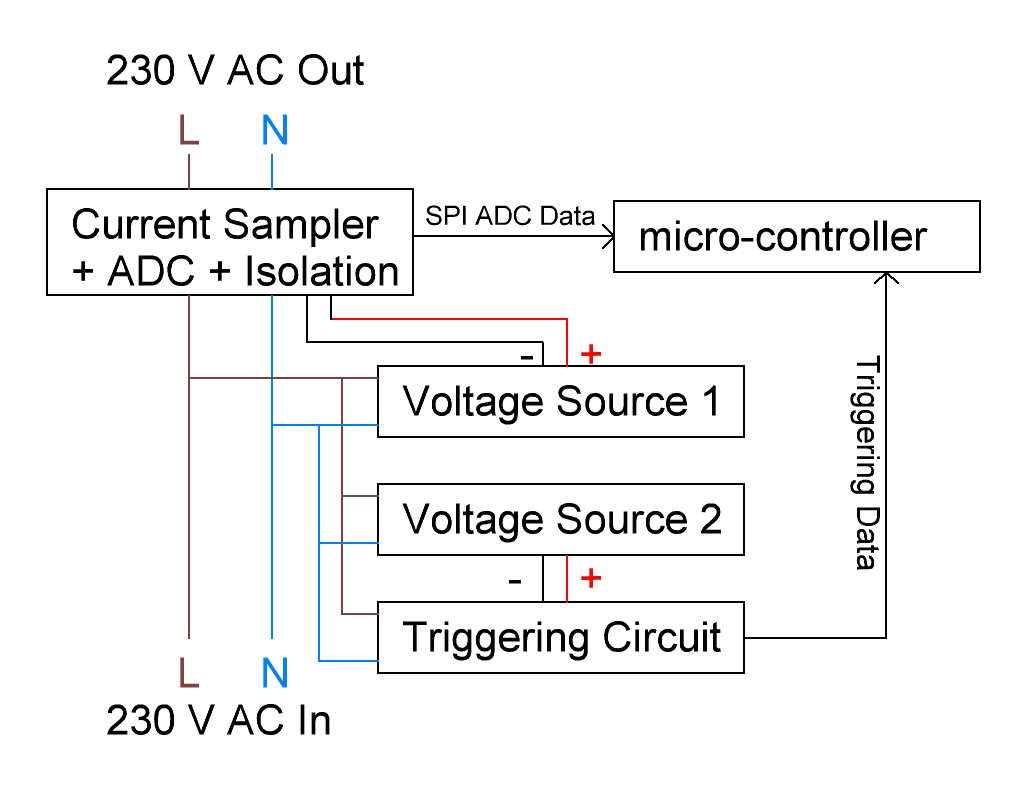
\includegraphics[angle=0,width=0.7\textwidth,keepaspectratio]{chapters/hardware-chapters/AC/ac-current-sampler/ac-current-sampler-architectural.JPG}
	\caption{Architectural overview of the AC current sampler.}
	\label{fig:ac-current-sampler-architectural}
\end{figure}


For the current-sampler itself a resistor will be used, since this approach ensures that no noise will be introduced to the sampled current signal.
As could be seen from \autoref{fig:custom-modulator-current-source}, the current that flows is both positive and negative, due to the nature of the AC that is used.
This means that the voltage that is measured over the resistor will also be positive and negative.
An ADC (Analog-to-Digital Converter) cannot measure a negative voltage.
So a constant offset voltage is summed with the voltage over the resistor to ensure that the ADC will always measure a positive voltage.
This offset voltage comes from a reference voltage IC \cite{lm336z-ref-voltage-datasheet}, which outputs a very stable reference voltage often used in scenarios where an ADC is used to measure analog signals.

At this point the ADC is measuring the voltage over a resistor which is in series with the ground (N) or phase (L) of the 230 V AC.
For safety reasons the ADC must now be electrically isolated from the micro-controller, such that no harm can come from even touching the micro-controller.
To this end, an SPI isolating chip was used \cite{iso7241m-spi-isolator-datasheet} to electrically isolate the SPI signals between the ADC and the micro-controller.




This solution to sample current with an external ADC can sample the current with a high frequency ($> 10$ kHz) with no noise introduced in the signal.
The full schematic of the current sampler can be found in \autoref{app:custom-current-sampler-schematic}.



